% Created 2019-04-02 Tue 13:38
% Intended LaTeX compiler: pdflatex
\documentclass[presentation]{beamer}
\usepackage[utf8]{inputenc}
\usepackage[T1]{fontenc}
\usepackage{graphicx}
\usepackage{grffile}
\usepackage{longtable}
\usepackage{wrapfig}
\usepackage{rotating}
\usepackage[normalem]{ulem}
\usepackage{amsmath}
\usepackage{textcomp}
\usepackage{amssymb}
\usepackage{capt-of}
\usepackage{hyperref}
\AtBeginSection[]{\begin{frame}<beamer>\frametitle{Topic}\tableofcontents[currentsection]\end{frame}}
\setbeamertemplate{caption}[numbered]
\usepackage{caption}
\captionsetup{font=scriptsize,labelfont=scriptsize}
\usetheme{default}
\author{Tim Sit}
\date{\today}
\title{Normative models of change detection}
\hypersetup{
 pdfauthor={Tim Sit},
 pdftitle={Normative models of change detection},
 pdfkeywords={},
 pdfsubject={},
 pdfcreator={Emacs 25.2.2 (Org mode 9.1.14)}, 
 pdflang={English}}
\begin{document}

\maketitle
\begin{frame}{Outline}
\tableofcontents
\end{frame}


\section{Overview}
\label{sec:orga96207b}

\begin{frame}[label={sec:orgec82ea3}]{Change detection}
\end{frame}

\begin{frame}[label={sec:orgbc1450f}]{Types of change detection}
Offline: 

\begin{itemize}
\item you have the entire dataset in your hands
\end{itemize}

Online: 

\begin{itemize}
\item you receive new data over time
\item often further divided into 
\begin{itemize}
\item batch detection: detect changes in batches of incoming data
\item sequential detection: detect changes with each new data point
\end{itemize}
\end{itemize}
\end{frame}

\begin{frame}[label={sec:org363ee1f}]{Types of models for change detection}
\begin{columns}
\begin{column}{0.5\columnwidth}
Frequentist methods 

\begin{itemize}
\item Changepoint model (Hawkins, Qiu, Kang 2003)
\end{itemize}
\end{column}

\begin{column}{0.5\columnwidth}
Bayesian methods

\begin{itemize}
\item Bayesian online changepoint detection (Adams and Mackay 2007)
\item Adaptive Sequential Bayesian Change Point Detection (Turner, Saatci, Rasmussen 2009)
\end{itemize}
\end{column}
\end{columns}
\end{frame}

\section{Bayesian online changepoint detection (Adams and Mackay 2007)}
\label{sec:org97dccbb}


\section{Examples}
\label{sec:org3e80f30}

\begin{frame}[label={sec:org1b220c1}]{Bayesian online change point detection (Adams and Mackay 2007)}
\begin{figure}[htbp]
\centering
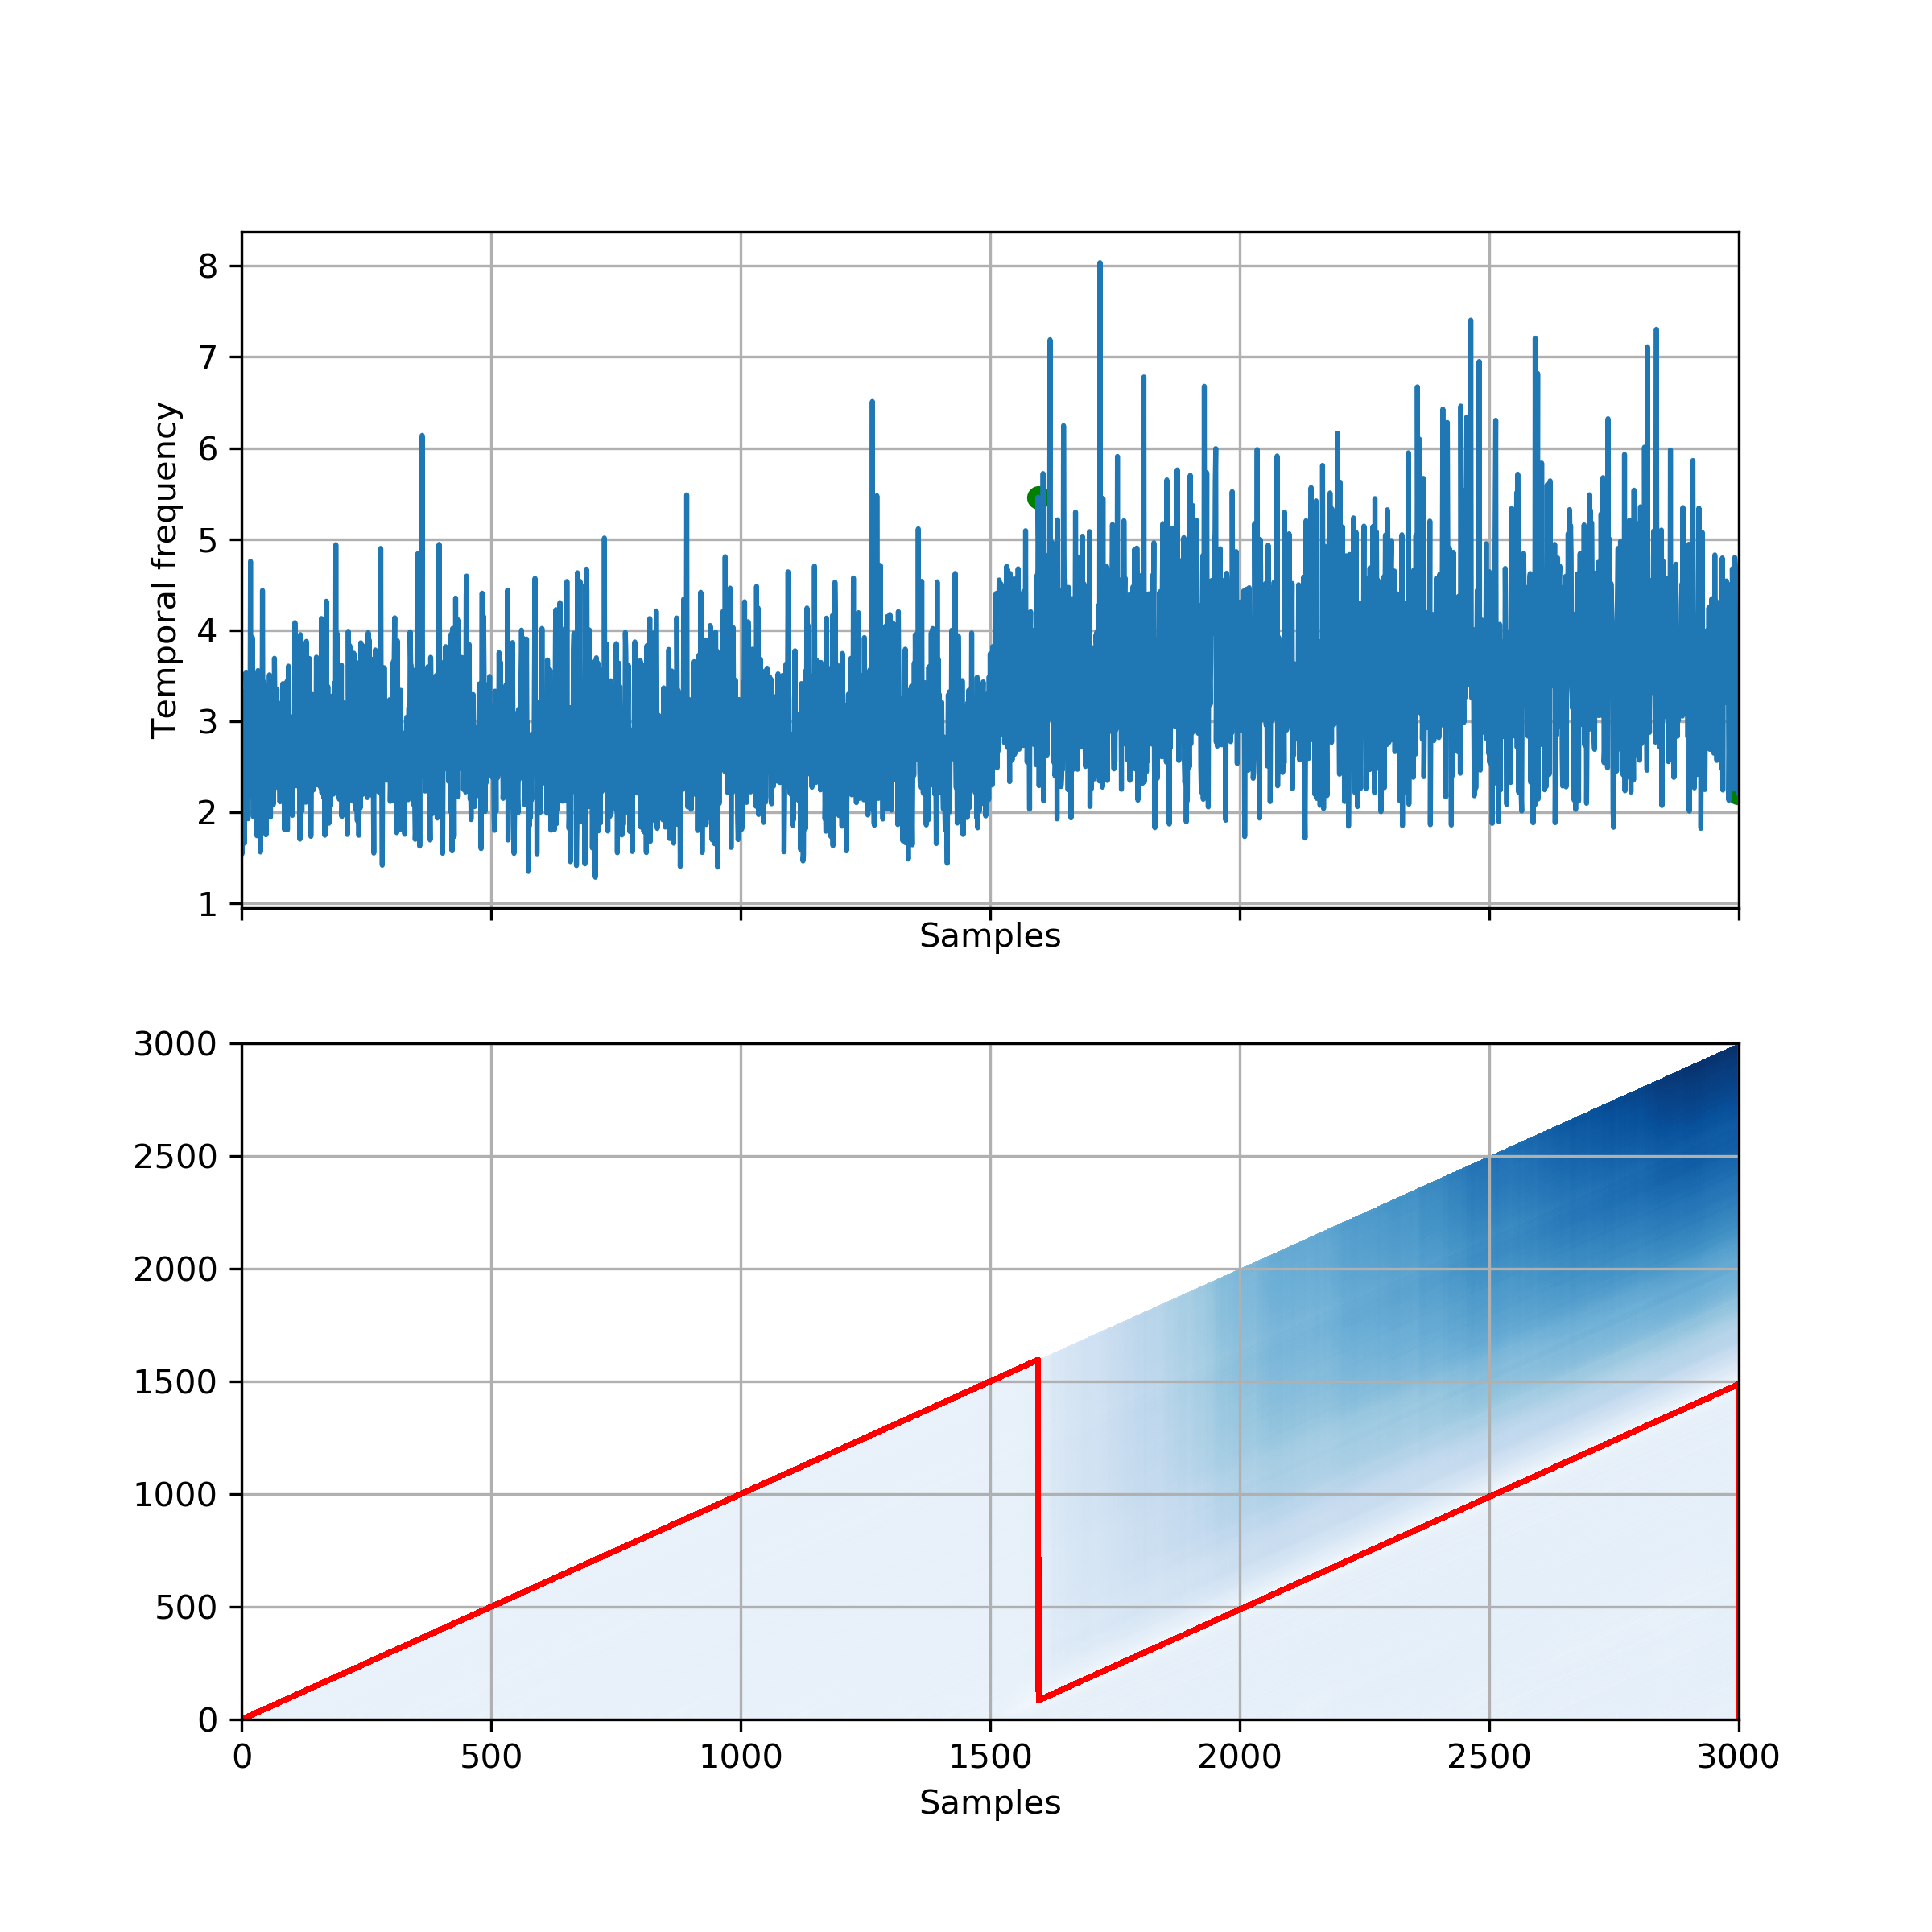
\includegraphics[width=0.55 \textwidth]{/home/timothysit/Dropbox/notes/Projects/second_rotation_project/normative_model/figures/test.png}
\caption{Single change point, two Gaussians with different means but equal variance}
\end{figure}
\end{frame}
\end{document}